\chapter{Theorie}
In diesem Kapitel werden die theoretischen Grundlagen für die Arbeit beschrieben.

Dabei werden zuerst die verschiedenen Graphenarten erläutert. Anschließend wird
der Stream-Prozess mit den verschiedenen Modellen beschrieben.

Danach folgt eine Vorstellung der verschiedenen Bibliotheken und welche
zugrundeliegende Streaming-Modelle dort zum Einsatz kommen.

Abschließend folgt ein Vergleich der verschiedenen Bibliotheken.

\section{Graphen}
Ein Graph G ist eine Datenstruktur mit der folgenden Definition: $G = (V,E)$.
Dabei ist V die Menge von Knoten und E die Menge von Kanten. Jede Kante besteht
dabei aus einem Paar von V. Bei einem ungerichteten Graphen ist das Paar, welches
die Kante repräsentiert, ein ungeordnetes Paar bzw. eine Menge von zwei
Elementen von V. Im Gegensatz dazu ist es bei einem gerichteten Graphen ein
geordnetes Paar.

\textquote[\cite{Aigner2015}]{
[\dots] Ein Graph $G = (V,E)$ besteht aus einer endlichen Menge V von Ecken,
einer endlichen Menge E von Kanten, und einer Vorschrift, welche jeder Kante e
genau zwei (verschiedene oder gleiche) Ecken a und b zuordnet, die wir die
Endecken von e nennen. Normalerweise sind die Endecken a und b verschieden;
ist a = b, so nennen wir e eine Schlinge bei a. Hat e die Endecken a und b, so
sagen wir, e verbindet a und b. [\dots]
}

Ein Weg ist eine Menge von Knoten mit der Bedingung, dass für alle Knoten eine
Kante gibt, welche zum nächsten Knoten führt. In der Regel sind Start- und
End-Knoten verschieden. Wenn Start- und End-Knoten gleich sind, handelt es sich
um einen Kreis. Zwei Sonderfälle von Kreisen spielen bei vielen Graph-Problemen
eine Rolle Schlingen und Mehrfachkanten. Schlingen sind Kreise der Länge eins.
Dies bedeutet, dass kein weiterer Knoten zwischen dem Start- und End-Knoten
liegt. Mehrfachkanten sind Kreise der Länge zwei. Dabei liegt noch genau ein
Knoten zwischen dem Start- und End-Knoten. Diese Kanten lassen sich zu einer
einzigen Kante zusammenfassen. Dazu wird nur eine Kante dargestellt mit einer
Zahl versehen, welche die Mehrfachkanten repräsentiert.

\textquote[\cite{Aigner2015}]{
Sind $v_{0}, v_{1}, v_{2}, \ldots, v_{t}$ Ecken mit $v_{i−1}v_{i} ∈ E$ für alle i,
so heißt $W = (v_{0}, v_{1} , \ldots, v_{t} )$ ein Kantenzug von $v_{0}$ nach
$v_{t}$ . Die Länge $l(W) = t$ des Kantenzuges ist die Anzahl der durchlaufenen
Kanten. W heißt ein Weg, falls alle $v_{i}$ verschieden sind. Es ist klar, dass
in jedem Kantenzug von a nach b ein a, b-Weg enthalten ist. Ein Kantenzug
$W = v_{0}, v_{1}, ... , v_{t}$, in dem alle Kanten verschieden sind und ebenso
alle Ecken mit Ausnahme $v_{0} = v_{t}$ , heißt ein Kreis, wobei t wiederum die
Länge des Kreises ist.
}

Es werden zwei Klassen von Graphen unterschieden. Graphen, welche nur keine
Schlingen und Mehrfachkanten zulassen, werden als einfache Graphen bezeichnet,
sonst als Multi-Graphen.

\textquote[\cite{Gurski2010}]{
[\dots] Kanten, die mit mehr als zwei Knoten inzident sind, werden Hyperkanten
genannt. Graphen mit Hyperkanten heißen Hypergraphen. Wir betrachten in diesem
Buch jedoch vorwiegend einfache Graphen, also Graphen ohne multiple Kanten und
ohne Schleifen, und auch keine Hypergraphen.
}

\section{Stream-Processing}
Stream-Processing beschreibt einen Prozess, bei dem die kontinuierlich
ankommenden Daten verarbeitet bzw. transformiert werden. Ein Stream ist eine
unendliche Liste von Elementen. Die Daten werden dabei von mindestens einer
Quelle gelesen. Anschließend werden diese von mindestens einer Verarbeitungseinheit
transformiert und abschließend in mindestens ein Ziel geschrieben. Quelle und
Ziel sind dabei externe Systeme, wie Datenbanken, Messaging-Platformen,~\dots,
welche in der Regel verschieden sind.

Die Idee des Stream-Processing ist schon sehr alt und im Laufe der Zeit sind
mehrere Modelle entstanden. Jedes Modell hat dabei gewisse Voraussetzungen
und Einschränkungen, welche direkten Einfluss auf die konkreten Umsetzungen
haben. Es gibt die Modelle \enquote{Classical Streaming}, \enquote{semi-Streaming},
\enquote{W-Stream} und \enquote{StreamSort}.

\subsection{Classical Streaming}
Das erste Modell ist das \enquote{Classical Streaming}. Dieses wurde in den
1980 von Munro und Paterson definiert. Das Modell beschreibt die Verarbeitung
eines Streams durch eine \gls{RAM}-Maschine. Der Stream ist dabei eine Folge von
Zeichen aus einem definierten Alphabet, welche sequenziell verarbeitet werden
können.

Die Prameter dieses Modells sind der Speicher der \gls{RAM}-Maschine in Bits und
die Anzahl der Verarbeitungsdurchläufe des Streams. Beide Parameter sind dabei
abhängig von der Länge des Streams und sollen möglichst klein im Verhältnis zur
Länge des Streams sein.

\foreigntextquote{english}[\cite{Ribichini2007}]{
In classical streaming, input data can be accessed sequentially in the form
of a data stream, and need to be processed using a working memory that
is small compared to the length of the stream. The main parameters of the
model are the number p of sequential passes over the data and the size s of the
working memory (in bits). [\dots]
}

Das Modell macht dabei keine Aussagen über die Laufzeit des Algorithmus. Diese
spielt für viele Probleme jedoch eine Rolle, deshalb wurde das
\enquote{semi-Streaming} Modell entwickelt.

\foreigntextquote{english}[\cite{Ribichini2007}]{
Notice that our definition imposes no restrictions on the amount
of computation performed by the RAM machine, as it is often the case when
dealing with external memory models, where it is assumed that I/O operations
take orders of magnitude longer than internal memory operations. There
are, however, applications in which the per-item processing time (average,
maximum) is a significant parameter that should be taken into account.
}

\subsection{semi-Streaming}
Das \enquote{semi-Streaming} Modell ist ein vereinfachtes Modell des
\enquote{Classical Streaming} Modells. Im Gegensatz zum \enquote{Classical Streaming}
wird hier festgelegt, das die Anzahl der Durchläufe beschränkt wird auf eins bzw.
einige wenige Durchläufe. Des Weiteren wird die Speichergröße der RAM-Maschine
beschränkt auf die logarithmische-Komplexitätsklasse.

\foreigntextquote{english}[\cite{Ribichini2007}]{
In particular, some recent papers show that several graph problems can be
solved with one or few passes in the Semi-streaming model [53] where the
working memory size is $O(n · \text{polylog} n)$ for an input graph with n
vertices (or even $O(n^{1 + \epsilon})$, with $\epsilon < 1$, for applications
like spanners, for which linear memory in the number of vertices is provably not
sufficient): [\dots].
}

Diese Beschränkungen sorgen dafür, dass die Laufzeit des Algorithmus verbessert
wird. Jedoch haben diese Beschränkungen auch den Nachteil, dass sie nur
näherungsweise Ergebnisse liefern.

\foreigntextquote{english}[\cite{Ribichini2007}]{
Despite the heavy restrictions of the classical streaming model, major
success has been achieved for several data sketching and statistics problems,
e.g., approximate frequency moments [7], histogram maintenance [58],
L\textsuperscript{1} difference [55], where $O(1)$ passes and polylogarithmic
working space have proven enough to find approximate solutions (see also the
bibliographies in [14, 88]).
}

\subsection{W-Stream}
Das \enquote{W-Stream} Modell oder \enquote{Write-Stream} Modell ist eine
Erweiterung des \enquote{Classical Streaming}. Dabei wird jedes gelesene Element
des Streams nach der Verarbeitung in einen Ausgabe-Stream geschrieben. Die
Elemente können dabei bevor sie in den Ausgabe-Stream landen, verändert werden.
Wenn die Elemente nicht verändert werden, handelt es sich um einen speziellen
\enquote{W-Strem}, nämlich den \enquote{Classical Stream}.

\foreigntextquote{english}[\cite{Ribichini2007}]{
In the W-Stream model [97], a streaming pass, while reading data from
the input stream and processing them in the working memory, produces items
that are sequentially appended to an output stream. [\dots]
Clearly, $\text{Stream}(p, s) \subseteq \text{W-Stream}(p, s)$ since at every
s/w-pass the output stream may simply consist of a copy of the input stream.
}

\subsection{StreamSort}
Das \enquote{StreamSort} Modell ist eine Erweiterung zum \enquote{W-Stream}.
Dabei schließt sich nach dem Schreibprozess noch ein Sortierungsprozess an. Dabei
werden die Elemente noch einer vorgegebenen globalen Sortierungsreihenfolge
sortiert.

\foreigntextquote{english}[\cite{Ribichini2007}]{
[\dots] This model extends classical streaming in two ways the ability to write
intermediate temporary streams and the ability to reorder them at each pass for
free. [\dots]
}

\section{Graph-Streaming Bibliotheken}
Graph-Streaming Bibliotheken sind Bibliotheken, welche die beiden Welten
\gls{BigData} und Graphen miteinander kombinieren wollen. Dabei geht es darum
große Graphen bzw. Teilgraphen effizient und möglichst in Echtzeit mit der Hilfe
von Streams zu verarbeiten.

Bevor eine Verarbeitung der Daten stattfinden kann, muss die Repräsentation
definiert sein. In unserem Fall sollen Streams verarbeitet werden, deren Daten
unseren Graphen repräsentieren. Um den Graphen darzustellen gibt es, mehrere
Möglichkeiten.

Die erste Möglichkeit ist es zwei separate Streams zu verwenden einen für die
Knoten und eine für die Kanten. Um eine Verarbeitung durchzuführen ist es bei
diesem Modell notwendig, die beiden Streams zu kombinieren.

\foreigntextquote{english}[\cite{Bali2015}]{
Combining edge and vertex streams The first approach was to have separate
edge and vertex streams. When we need to know the vertex values corresponding
to the end points of an edge, the two streams can be joined.
}

Eine andere Möglichkeit ist es die Werte der beiden Knoten und die dazugehörige
Kante mit abzuspeichern. Das Problem bei dieser Darstellung ist allerdings, 
falls nicht alle Daten der Knoten vorhanden sind, entstehen Fehler.

\foreigntextquote{english}[\cite{Bali2015}]{
Triplet stream Another way to stream graphs would be the use of triplets.
Triplets are pairs of vertices around an edge. Both the edge and the two vertices
can have their own value.
}

Die einfachste Möglichkeit besteht darin einfach ein Stream aus Knotenpaaren zu
nehmen, welche genau eine Kante repräsentieren.

\foreigntextquote{english}[\cite{Bali2015}]{
Edge-only stream The final model we considered is the simplest. The graph
consists of a single stream of edges.
}

Allerdings gibt es bei allen Darstellungsformen einige Probleme. Zunächst einmal
gibt es keine Information, ob es sich um einen ungerichtete oder gerichtete
Kante handelt. Des Weiteren existiert auch keine Statusinformation über die
Änderung der Kante bzw. über den Grund was zum Erzeugen der Kante geführt hat
z. B. wurde die Kante oder ein Knoten hinzugefügt, gelöscht, geändert,~\dots .
Ein anderes Problem tritt auf, wenn nur ein Knoten hinzugefügt wird, wie wird
dieser dann dargestellt bzw. verarbeitet. Außerdem stellt sich die Frage, wie
gewichtete Graphen dargestellt werden, welche bei der Routenplanung zum Einsatz
kommen.

Die Funktionalität der Bibliotheken richtet sich auch nach dem zugrundeliegende
Streaming-Modell bzw. der Laufzeitumgebung. In dieser Arbeit werden die
Bibliotheken \enquote{gelly-streaming}, \enquote{graphstream-project} und
\enquote{Gephi} verglichen.

\subsection{gelly-streaming}
\enquote{gelly-streaming} ist eine Graph-Streaming Bibliothek für Apache Flink\footnote{\url{https://flink.apache.org}}.
Diese wurde von Vasiliki Kalavri am KTH in Schweden im Jahr 2015 entwickelt.
Sie ist in der Programmiersprache Java geschrieben und besitzt auch kein andere
Schnittstelle. Derzeit ist die Bibliothek noch in einem experimentellen Stadium,
deshalb gibt es noch keine Alpha/Beta/Finale-Versionen. Die Bibliothek verwendet,
dass semi-Streaming Modell. Bei dem nur der Stream aus Kanten abgespeichert wird.
Die Kante wird dabei durch zwei Knoten representiert. Die Bibliothek ist dabei
in ihrer Funktionalität gebunden, an ihre Laufzeitumgebung
Apache-Flink, deren \gls{API} sie benutzt. Derzeit wird Apache Flink 1.2.0 benutzt.

\foreigntextquote{english}[\cite{Bali2015}]{
The semi-streaming model allows for the storage of O(polylog n) elements for n
edges, and also O(polylog n) passes. Since we cannot have multiple passes in our
model, we use a modified semi-streaming model. Not every algorithm of the
semi-streaming model will be possible to implement in our model.
}

Apache Flink eine verteilte Plattform für Batch- und Stream-Processing. Der Kern
von Apache Flink ist die Streaming-Engine, welche die eigentliche Verarbeitung
der Daten vornimmt. Apache Flink wurde in der Programmiersprache Java an der TU
Berlin entwickelt und ist jetzt ein Apache Projekt. Zusätzlich zur Java-\gls{API}
existiert noch eine Scala-\gls{API}, welche als Wrapper dient. Die aktuelleste
Version ist 1.6.0. Apache Flink wird hauptsächlich von der Firma \enquote{data Artisans}
weiterentwickelt. Diese veranstalltet auch Konferenzen um mit der Community in
verbindung zu bleiben und dort neue Impulse anzuregen. Im Jahr 2019 wurde die
Firma von \enquote{Alibaba} gekauft \cite{Parbel2019}. In wie weit dies Einfluss
auf die weitere Entwicklung von \enquote{gelly-streaming} nehmen wird lässt sich
zum jetzigen Zeitpunkt nicht sagen.

Apache Flink ist modular aufgebaut. Die Architektur ist im Bild \ref{fig:flink-architecture}
dargestellt. Auf die Streaming-Engine bauen die beiden \gls{API} auf.
Die \enquote{DataStream-API} definiert die verschiedenen Schnittstellen und Klassen
für Streams. Die \enquote{DataSet-API} definiert die verschiedenen Schnittstellen
und Klassen für Datenfelder bzw. Listen. Diese werden dabei von der Engine in
endliche Streams umgewandelt.

\begin{figure}
\centering
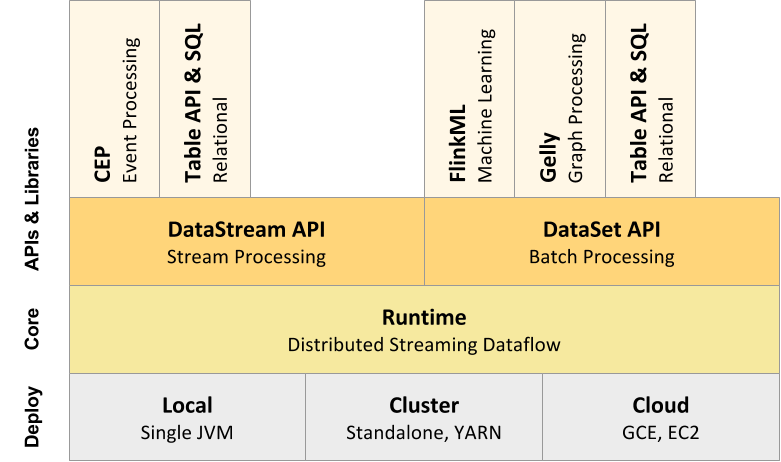
\includegraphics[height=10cm, width=15cm]{../material/images/flink-stack-graphic.png}
\caption{Architektur von Apache Flink \cite{Foundation2018}}
\label{fig:flink-architecture}
\end{figure}

\foreigntextquote{english}[\cite{Foundation2018}]{
The basic building blocks of Flink programs are streams and transformations.
(Note that the DataSets used in Flink’s DataSet API are also streams internally
– more about that later.) Conceptually a stream is a (potentially never-ending)
flow of data records, and a transformation is an operation that takes one or
more streams as input, and produces one or more output streams as a result.

When executed, Flink programs are mapped to streaming dataflows, consisting of
streams and transformation operators. Each dataflow starts with one or more
sources and ends in one or more sinks. The dataflows resemble arbitrary
directed acyclic graphs (DAGs). Although special forms of cycles are permitted
via iteration constructs, for the most part we will gloss over this for
simplicity.
}

\subsection{graphstream-project}
\enquote{graphstream-project} ist eine Java-Bibliothek für Graph-Streaming. Die
Bibiliothek wurde 2009 von der Gruppe RI\textsubscript{2}C-Gruppe am LITIS ein
Zusammenschluss von mehreren Universitäten und Firmen entwickelt. Derzeit wird
die Bibliothek von der Universität Le Havre weiterentwickelt. Die aktuellste
Version ist 1.3 .

Die Bibliothek besteht aus drei verschiedenen Modulen core, algo und ui. Das
core-Modul enthält alle Basisklassen zum Lesen und Anzeigen von Graphen. Das
algo-Modul enthält zusätzliche Algorithmen für Graphen. Das ui-Modul enthält ein
alternatives Framework zur Darstellung der Graphen.

\foreigntextquote{english}[\cite{Team2018}]{
gs-core is the base of GraphStream which is all you need to read a graph and
display it easily. gs-algo contains extra algorithms which can be run on a graph.
gs-ui provides other graphic viewers and will contain sources for graphical tools.
}

Das Bild \ref{fig:graphstream-project-architecture} zeigt einen beispielhaften
Ablauf eines Verarbeitungsprozesses. Der Graph wird aus einer Datei gelesen und
die erzeugten Events stellen das Ziel dar. Diese Events sind gleichzeitig die
Quelle der Verarbeitungseinheit, welche wiederum neue Events erzeugt. Diese neuen
Events stellen die Quelle für die Ausgabe dar. Das verwendete Streaming-Modell
wird dabei nicht erwähnt. Aufgrund der Tatsache, dass die Bibliothek sowohl
Einfache- als auch Multi-Graphen abdecken kann, ist es aber wahrscheinlich, dass
\enquote{Classical Streaming} zum Einsatz kommt.

\foreigntextquote{english}[\cite{Team2018}]{
GraphStream is a graph handling Java library that focuses on the dynamics aspects
of graphs. Its main focus is on the modeling of dynamic interaction networks of
various sizes.

The goal of the library is to provide a way to represent graphs and work on it.
To this end, GraphStream proposes several graph classes that allow to model
directed and undirected graphs, 1-graphs or p-graphs (a.k.a. multigraphs, that
are graphs that can have several edges between two nodes).

GraphStream allows to store any kind of data attribute on the graph elements:
numbers, strings, or any object.

Moreover, in addition, GraphStream provides a way to handle the graph evolution
in time. This means handling the way nodes and edges are added and removed, and
the way data attributes may appear, disappear and evolve.
}

\begin{figure}
\centering
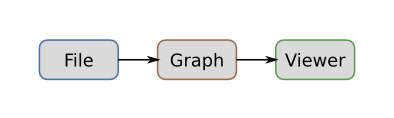
\includegraphics[width=15cm]{../material/images/graphpipeline-graphstream.png}
\caption{Architektur von graphstream-project \cite{Team2018}}
\label{fig:graphstream-project-architecture}
\end{figure}

\subsection{Gephi}
\enquote{Gephi} ist eine Visualisierungsplatform für Graphen, welche in Java
geschrieben ist. Diese wurde 2009 an der Universität of Technologie of Compiègne
in Frankreich entwickelt. Derzeit wir die Platform vom Gehpi Consortium betreut.
Die aktuelleste Version ist 0.9.2 .

Die Bibliothek baut auf der Netbeans Platform auf. Das Programm bietet dabei nur
die Basisfunktionalität an. Zusätzliche Funktionen werden durch Plug-Ins
realisiert. Die Streaming-Funktionalität besteht aus zwei Teilen, dem Client und
Server. Die Kommunikation erfolgt dabei in der Regel über \gls{JSON}.

\foreigntextquote{english}[\cite{Bastian2009}]{
Gephi Graph Streaming is divided in different modules: The core modules, that
defines the Graph Streaming API and its implementation, the Server modules,
responsible for the HTTP REST Server, and the interface modules. 
}

\enquote{Gephi} macht über das Streaming-Modell ebenfalls keine genauen Angaben.
Da \enquote{Gephi} wie auch \enquote{graphstream-project} Events für
Knotenerzeugung und extra Angaben wie Gewichte,~\dots erlaubt, ist hier
ebenfalls von einem \enquote{Classical Streaming} Modell auszugehen.

\section{Vergleich der Bibliotheken}
Nachdem die Bibliotheken vorgestellt wurden, soll nun ein Vergleich erfolgen.
Dabei soll das Augenmerk auf folgenden Punkten liegen:

\begin{itemize}
\item Generatoren
\item Algorithmen
\item Verteilung
\item Connectoren
\end{itemize}

\subsection{Generatoren}
Die Verwendung von Generatoren ist gerade bei der Entwicklung von Programmen
wichtig. Wenn noch kein sehr großes Verständnis oder Datenbasis des angestrebten
Zieles vorhanden ist, der Entwickler jedoch schon die Funktionalität seines
Algorithmus testen möchte. Generatoren bieten sich im Allgemeinen an, wenn die
eigentliche Zielerzeugung zu aufwendig ist oder aus anderen Gründen nicht möglich
ist z. B. wenn ein externes System beteiligt ist. Generatoren bieten den
Vorteil, dass die Struktur vorgeben werden kann und die konkrete Ausprägung jedoch
immer zufällig ist. Auf die Bibliotheken bezogen bedeutet dies, die Struktur ist
z. B. ein einfacher Graph mit sieben Knoten und die konkrete Ausprägung sind dann
die Kanten, welche zufällig verteilt sein können.

\enquote{gelly-streaming} hat als einzige Bibliothek keinen Generatoren.
Die \enquote{Gelly} die Batch-Processing Bibliothek von Apache Flink hat mehrere
Generatoren.

\foreigntextquote{english}[\cite{Foundation2018}]{
Gelly provides a collection of scalable graph generators. Each generator is

\begin{itemize}
\item parallelizable, in order to create large datasets
\item scale-free, generating the same graph regardless of parallelism
\item thrifty, using as few operators as possible
\end{itemize}

Graph generators are configured using the builder pattern. The parallelism of
generator operators can be set explicitly by calling setParallelism(parallelism).
Lowering the parallelism will reduce the allocation of memory and network buffers.

Graph-specific configuration must be called first, then configuration common to
all generators, and lastly the call to generate(). The following example
configures a grid graph with two dimensions, configures the parallelism, and
generates the graph.
}

\enquote{graphstream-project} hat die folgenden Generatoren:

\begin{itemize}
\item Flower Snark generator
\item Full connected graph generator
\item (Incomplete) grid generator
\item Lobster generator
\item etc.
\end{itemize}

Bei \enquote{Gephi} können die Generatoren je nach Anforderung selbst
programmiert werden. Aufgrund der zugrundeliegende Plugin-Architektur.

\foreigntextquote{english}[\cite{Bastian2009}]{
Generator API/SPI provides the way to create and execute graph generators.

Generators are tasks that create a graph structure from various properties.
New generators can be easily created, they will be automatically integrated.
}

\subsection{Algorithmen}
Die Algorithmen stellen die eigentliche Funktionalität der Bibliotheken dar.
Dabei wird unterschieden zwischen Basisfunktionen und Komplexfunktionen.
Zu den Basisfunktionen gehören:

\begin{itemize}
\item Abfragen von Eigenschaften
\item Transformation eines Streams
\item Berechnung von statistischen Werten
\item etc.
\end{itemize}

Komplexfunktionen kombinieren mehrere Basisfunktionen, um eine komplexe Funktion
durchzuführen. Die Algorithmen sind dabei abhängig, vom der Darstellung
des Graphen Streams, des Streaming-Modells, der Umgebung,~\dots .

\enquote{gelly-streaming} stellt verschiedene Basisfunktionen bereit und die
folgenden Algorithmen bereit: \cite{Kalavri2018}

\begin{itemize}
\item Connected Components
\item k-Spanner
\item Bipartiteness Check
\item Window Triangle Count
\item Triangle Count Estimation
\item Weighted Matching
\item Continuous Degree Aggregate
\end{itemize}

Weitere Algorithmen lassen sich je nach Anwendungsfall umsetzen, zum Beispiel um
den Stream zu filtern oder eine besondere Aggretationsfunktion zu implementieren.

\enquote{gelly-streaming} ist jedoch in ihrere Auswahl an Algorithmen eingeschränkt,
da ein abgeschwächtes \enquote{semi-Streaming} Modell zum Einsatz kommt. Bei dem
im Gegensatz zum theoretischen Modell keine mehrfachen Durchläufe gestattet sind.

\enquote{graphstream-project} stellt ebenfalls mehrere Algorithmen bereit wie:

\begin{itemize}
\item Betweenness Centrality
\item Closeness
\item Diameter
\item Clustering Coefficient
\item PageRank
\item Community detection (Modularity)
\end{itemize}

Weitere Algorithmen lassen sich durch Implementierungen eines Interfaces umsetzen.
Die Implementierung bekommt eine Referenz auf den Graphen, über eine
Initialisierungs-Methode, um eventuelle Vorbereitungen durchzuführen. Die
eigentliche Verarbeitung erfolgt in einer anderen Methode.

\enquote{Gephi} stellt verschiedene Methoden zur Abfrage des Graphen bereit.
Dabei wird zwischen statischer und dynamischer Abfrage unterschieden. Eine
dynamische Abfrage kann auch nur auf einem dynamischen Graphen durchgeführt
werden. Weitere Algorithmen können über Plug-Ins realisiert werden.

\subsection{Verteilung}
Verteilung kann für verschiedene Bereiche angewendet werden z. B. lassen sich
größere Datenpakete teilen, Algorithmen auf mehrere Prozesse verteilen, Programme
auf mehrere Rechner verteilen,~\dots . In unserem Fall ist die Verteilung der
Streaming-Programme auf mehrere Rechner gemeint.

\enquote{gelly-streaming} ist die einzige Bibliothek, welche verteilt auf mehrere
Knoten läuft, weil die Laufzeitumgebung Apache Flink dies unterstützt.
Der Cluster kann dabei in den verschiedensten Umgebungen laufen wie: \cite{Foundation2018}

\begin{itemize}
\item AWS
\item Docker
\item Kubernetes
\item etc.
\end{itemize}

Anwendungen von \enquote{graphstream-project} können nicht verteilt werden,
obwohl sie von der Art und Weise ähnlich aufgebaut sind wie Apache Flink Anwendungen.
Denn sie werden ebenfalls über die main-Methode aufgerufen.

\enquote{Gephi} Anwendungen lassen sich ebenfalls nicht, verteilen, dies hängt
damit zusammen, dass Gephi sich nur mit der graphischen Oberfläche gestartet
werden kann.

\subsection{Connectoren}
Connectoren sind der entscheidende Punkt, wenn es darum geht verschieden Systeme
miteinander zu verbinden. Dies ist gerade beim Streaming entscheidend, da die
Daten ja in Echtzeit von verschiedenen Systemen gelesen und wieder geschrieben
werden sollen.

Apache Flink unterstützt Connectoren. Dabei werden einige Connectoren
für Dateien, Sockets,~\dots vom Kern bereitgestellt. Zusätzliche Connectoren
werden über Bibliotheken bereitgestellt.

In der \enquote{graphstream-project} Bibliothek ist dies einfach Umzusetzen, da
die Connectoren, dort nur einfache Interface Implementierungen sind und diese
mit dem Graphen verbunden werden. Die bedeutet, wenn für ein spezielles
System eine Client-Bibliothek existiert, dann lässt sich ein Connector mit der
Hilfe der Client-Bibliothek programmieren.

Bei \enquote{Gephi} sind alle Erweiterungen Plug-Ins. Die dann entweder von der
Anwendung oder von anderen Plug-Ins benutzt werden können. Dies bedeutet es ist
grundsätzlich möglich, ein Plug-In zu schreiben, welches eine Verbindung zum
Beispiel zu Apache Kafka bereitstellt. Dies ist vom Streaming-Plug-In auch schon
für HTTP-Dienst so umgesetzt. Dabei existieren zwei Möglichkeiten. Die erste
Möglichkeit ist, dass \enquote{Gephi} als Client funktioniert und sich beim
externen Dienst anmeldet und dieser dann die Daten periodisch sendet. Dies ist
ähnlich wie bei WebSockets. Eine andere Möglichkeit ist, das \enquote{Gephi}
selbst als Dienst bzw. Master auftritt und sich sowohl externe Dienste wie auch
andere \enquote{Gephi}-Anwendungen dort anmelden können. Anschließend übernimmt
der Master die Kommunikation der einzelnen Teilnehmer. Dabei werden alle gesendeten
bzw. getätigten Änderungen an alle anderen Teilnehmer gesendet. Diese können
auf die eingehenden Ereignisse reagieren. Der Standardfall ist, dass einfach der
Graph aktualisiert wird.

Nachdem in diesem Kapitel die theoretischen Grundlagen gelegt wurden, wird in den
nächsten Kapiteln die einzelnen Bibliotheken miteinander an einem konkreten Beispiel
verglichen. Dabei stellt gelly-streaming die Referenz-Implementierung dar.
